\documentclass[12pt, letterpaper]{article}
\usepackage{graphicx}
\usepackage{hyperref}
\usepackage{amssymb}
\usepackage{amsmath}
\usepackage{float}
\usepackage{mathtools}
\usepackage{enumitem}
\usepackage[margin=1in]{geometry}
\usepackage[figurename=Figura]{caption}

\title{%
  Situación Problema: Análisis de Audio usando Fourier \\
  \large F1009: Análisis de métodos matemáticos para la física}

\begin{document}

\maketitle

\begin{tabular}{ccc}
Juan Pablo Guerrero Escudero & Romina Nájera Fuentes & Juan Braulio Olivares Rodríguez
\end{tabular}

\section{Introducción}

\section{Teoría}

\subsection{Conceptos físicos}

\subsubsection{Ondas de sonido}
De acuerdo a Young y Freedman \cite{university-physics}, El sonido se define como una onda 
longitudinal en un medio, principalmente aire, pero puede ser otros como otros gases, líquidos o sólidos. Las 
ondas de sonido más simple son ondas sinusoidales con una frecuencia, amplitud y longitud definida. 
\cite{university-physics}. El ser humano es capaz de escuchar ondas en el rango de 20 a 20,000 Hz, con 
frecuencias por encima del rango (ultrasónicas) o debajo del rango (infrasónicas) fuera del rango de escucha humano. 
De acuerdo a Hwaitat \cite{frequencies-wave-sound-pso}, las ondas de sonido son peturbancias propagadas por un medio el cuál 
no se ve afectado, y éstas ondas pueden ser ya sea longitudinales, o transversales. Para una onda 
de tipo longitudinal, el medio vibra en ángulos rectos al movimiento de la onda, y en el caso de ondas longitudinales, 
el medio vibra en la misma dirección que el movimiento.En la Figura \ref*{Ondas Longitudinales} se observa gráficamente lo discutido. 
\begin{figure}[H]
  \centering
  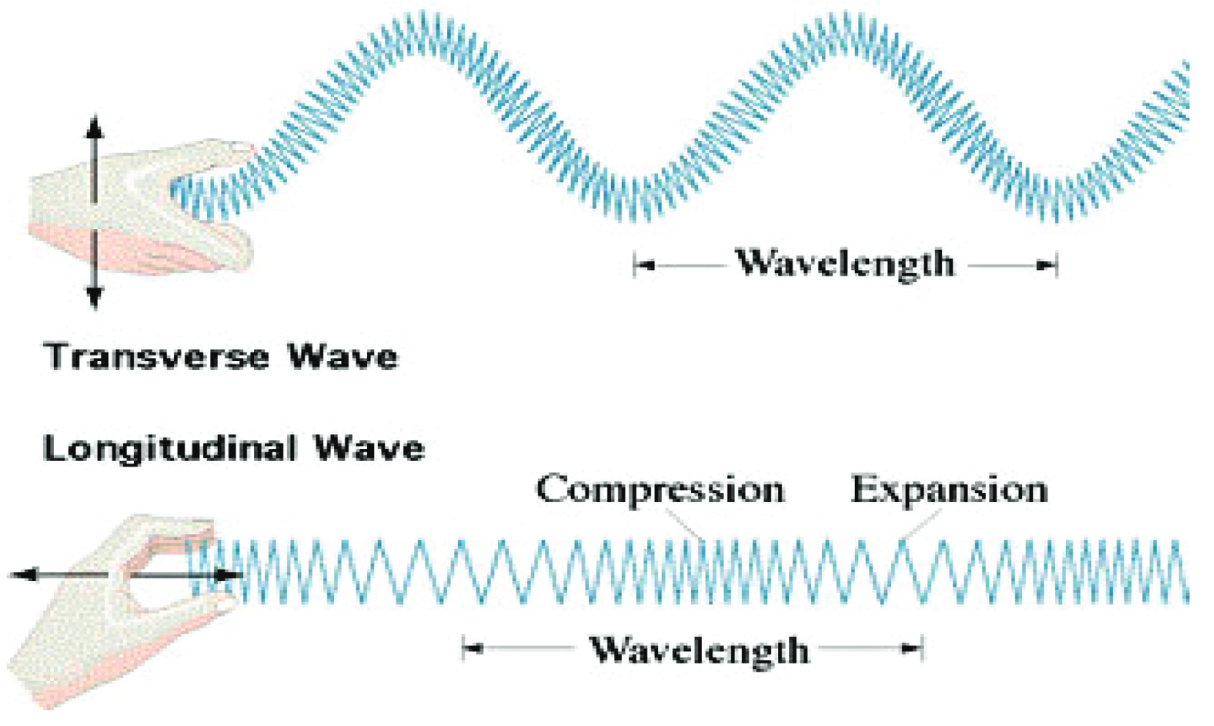
\includegraphics[height = 4cm]{ondas_longitudinales_transversales.png}
  \caption{Ondas longitudinales y transversales}
  \label{Ondas Longitudinales}
\end{figure}
Los parámetros de cualquier onda constituyen la amplitud, la frecuencia 
y la longitud, mencionados anteriormente. La amplitud puede ser definida como la "altura" 
de la onda, la frecuencia se define como los ciclos por segundo, y la longitud se define como la distancia 
entre un pico de onda y otro. Para una vista gráfica, vea la Figura \ref*{parametros-ondas}. Generalmente, sucede que 
cuando dos partículas están en movimiento en el mismo medio, ocurre interferencia. Ésto significa que 
las amplitudes de onda son sumadas algebraicamente, y se siguen moviendo por el medio sin distracciones. En el mundo real, 
la interferencia de ondas crea patrones complejo, y puede ser muy difícil de analizar.  
\begin{figure}[H]
  \centering
  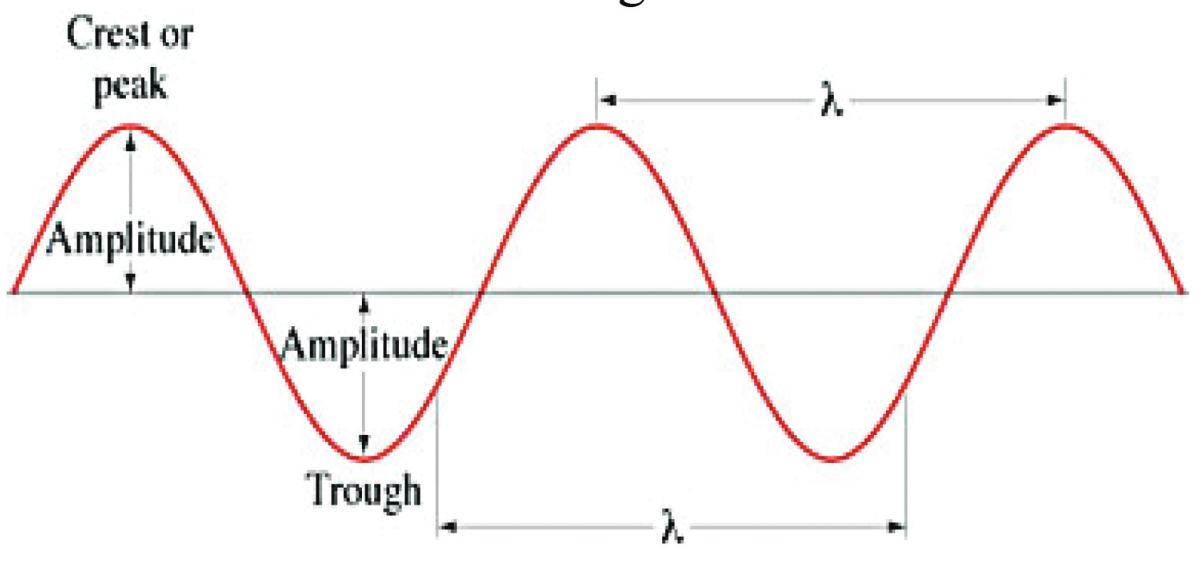
\includegraphics[height = 4cm]{parametros-ondas.png}
  \caption{Parámetros de las ondas de sonido}
  \label{parametros-ondas}
\end{figure}
\subsubsection{Frecuencias de audio/sonido}
Como se definió anteriormente, la frecuencia de una onda es, de acuerdo a [1], como el número de repeticiones 
de una función periódica durante una unidad de variación en la variable independiente. En otras palabras, es el número de 
ocurrencias de un evento repetitivo por unidad de tiempo. 
\subsubsection{Sonidos armónicos}
\subsubsection{Beats}

\subsection{Análisis de las canciones}

Para la clasificación de las canciones entre los géneros de música instrumental o reggaetón,
realizaremos un análisis espectral, el cual busca descomponer una serie de tiempo en las
ondas senoidales que la conforman \cite{Montenegro-2009}. Este análisis permitirá obtener las
diferentes frecuencias que conforman al pedazo de canción a analizar, y poder sacar conclusiones
sobre el género de la canción. \medskip

\noindent Para ello, utilizaremos la transformada de Fourier, utilizada
comúnmente en el campo científico, como en la acústica y el procesamiento de señales.
Esta herramienta transforma el dominio de una señal, pasando del tiempo a la frecuencia,
sin alterar su contenido \cite{Bernal-1999}.
Al perderse la noción del tiempo, analizaremos los rangos de frecuencias en los
que se encuentran magnitudes más grandes, para así identificar si la canción presentada
es instrumental o reggaetón.

\subsubsection{Transformada de Fourier}

Por definición, la transformada de Fourier de una función $f(x)$ es dada por la ecuación \ref{eq:fourier}
\begin{align}
	\phi_f(\alpha) &= \int_{-\infty}^{\infty} e^{i\alpha x} f(x) dx
	\label{eq:fourier}
\end{align}

\noindent Esta transformada fue desarrollada por Jean-Baptiste Joseph Fourier en el siglo XIX,
quien inició proponiendo que cualquier función arbitraria de una variable
podía ser expresada como una combinación lineal de funciones de senos y cosenos,
que son las series de Fourier \cite{OGorman-2023}. \medskip

\noindent A través de esas series, logró sintetizar la transformada, la cual
es distinguida por:
\begin{itemize}
  \item Determinar qué frecuencias están presentes en una señal.
  \item Transformar una señal del dominio temporal al dominio de frecuencia y viceversa.
\end{itemize}

\noindent Así como las series de Fourier descomponen una función en senos y cosenos, la
transformada descompone una señal en sus frecuencias, y aquellas que tengan una mayor
amplitud, se verán representadas como picos más altos, así como se puede observar en
la figura \ref{fig:fourier}.

\begin{figure}[H]
  \centering
  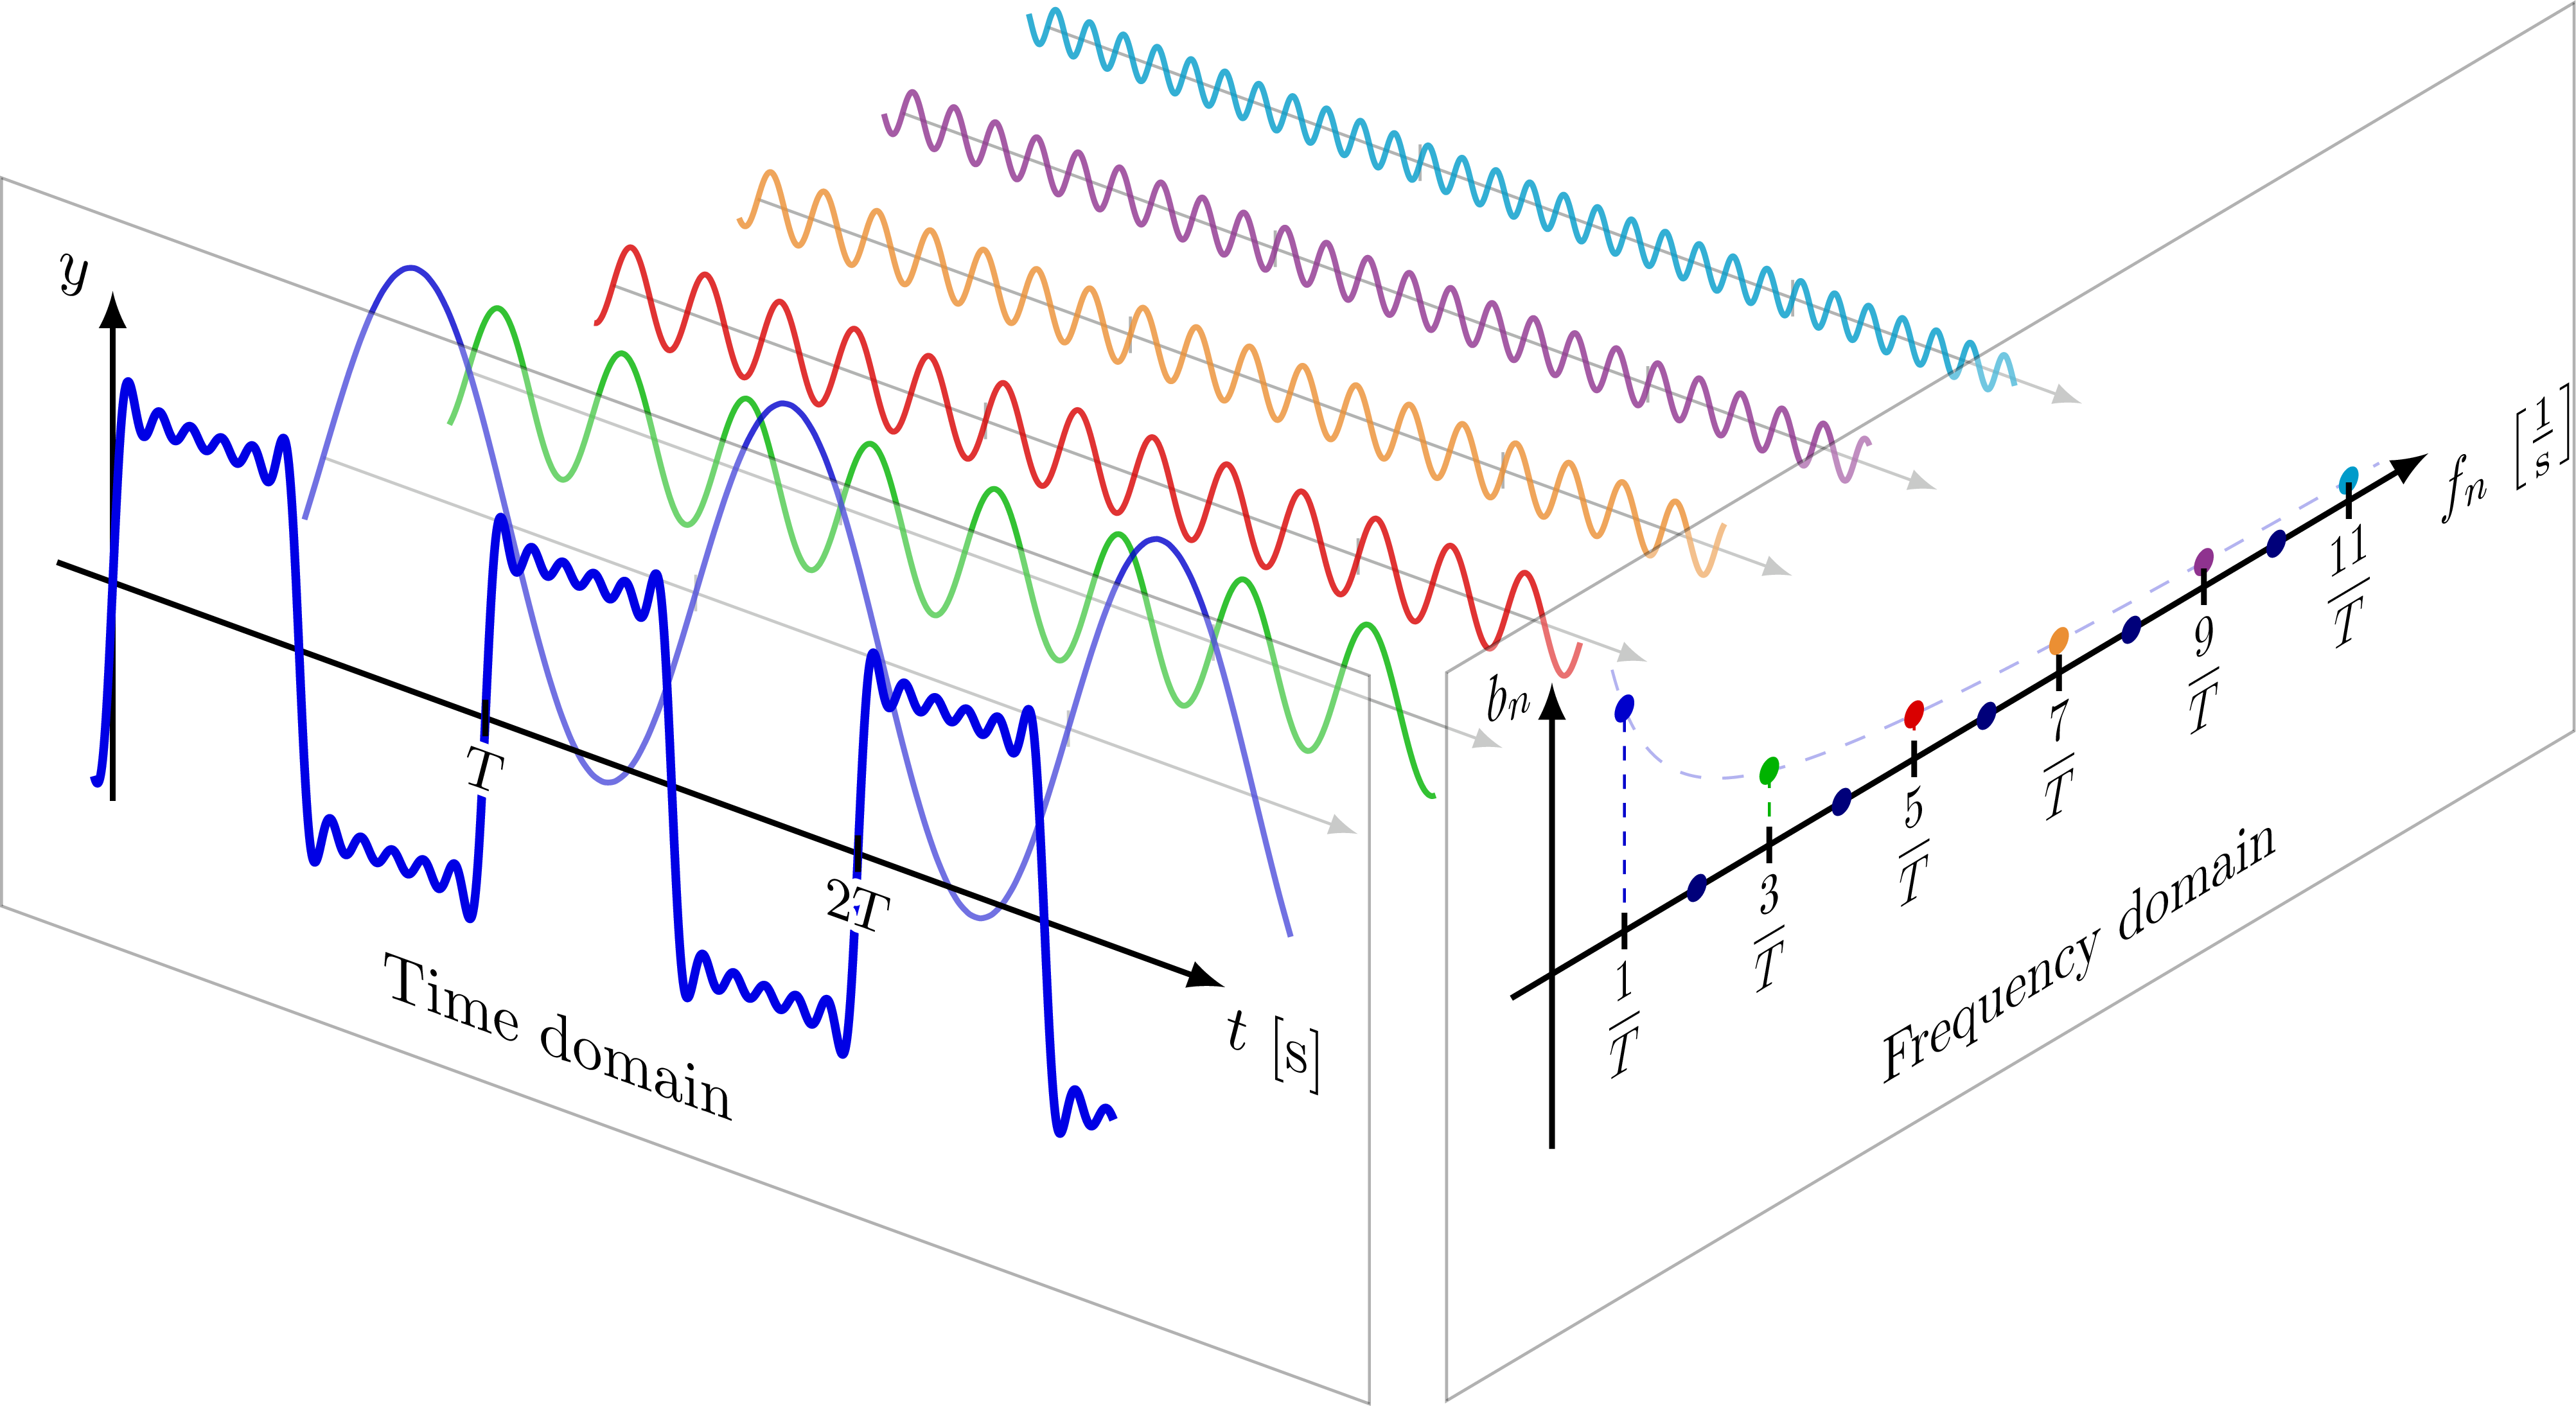
\includegraphics[width=0.9\textwidth]{FourierSeries_Freq.png}
  \caption{Representación visual de la transformada de Fourier \cite{OGorman-2023}.}
  \label{fig:fourier}
\end{figure}

\subsubsection{Espectrogramas}



\subsubsection{Rangos de frecuencias}

\section{Resultados}

\section{Conclusiones}



\begin{thebibliography}{9}
  \bibitem{university-physics}
  H. D. Young and Roger A. Freedman, \emph{University Physics with Modern Physics}, 
  Addison-Wesley, San Francisco, 2012. %%Para citar \cite{university-physics}
  \bibitem{frequencies-wave-sound-pso}
  Al Hwaitat et Al, Journal of Experimental \&\ Theoretical Artificial Intelligence,
  2022, 34, 749-780
  \bibitem{Montenegro-2009}
  A. Montenegro, \textit{CORE}, 2009, \url{https://core.ac.uk/download/pdf/6448967.pdf}
  \bibitem{Bernal-1999}
  J. Bernal, P. Gómez y J. Bobadilla, \textit{Estudios de fonética experimental}, 1999, \textbf{10}, 75-105.
  \bibitem{OGorman-2023}
  L. O'Gorman, \textit{DIBS Methods Meetings}, 2023, \url{https://dibsmethodsmeetings.github.io/fourier-transforms/}
\end{thebibliography}
\end{document}
